\documentclass[a4paper]{scrartcl}
\usepackage{mystyle1}
\usepackage{bm}
\usepackage{tikz}
\usepackage{dashrule}
\usepackage{listings}
\usepackage{array}
\usepackage{microtype}
\usepackage{mathtools}
\usepackage[left=2cm, right=2cm, top=2cm, bottom=2cm]{geometry}
%\usepackage{adjustbox}
%\usepackage{mathrsfs}
%\usepackage{cancel}
\usepackage{hyperref}
\hypersetup{
        colorlinks=true,
        urlcolor=RubineRed,
        linkcolor=RoyalBlue!90!black,
        citecolor=retrocyan,
        breaklinks=true
    }

    \usepackage[T1]{fontenc}   
    \usepackage{lmodern}    


\addtokomafont{title}{\sffamily}
\setkomafont{subtitle}{\LARGE\sffamily\bfseries}
%\DeclareFontShape{T1}{cmss}{b}{n}{<->ssub*cmss/bx/n}{}
\setkomafont{author}{\large}
\setkomafont{date}{}


\title{
        \Large\textsc{CS3101 Project: Flight Reservation System} \\
        \vspace{10pt}
        \Huge\textbf{Ronway Airlines} \\
}

\author{Ronit Bhuyan \\ \texttt{22MS025} \and Sagnik Seth \\ \texttt{22MS026} \and   Aviyank Aryan \\ \texttt{22MS030}}
\date{}







\begin{document}
\maketitle
\begin{figure}[H]
    \centering
    
\includegraphics[scale=0.3]{airplane.jpg}
\end{figure}
\pagebreak
\tableofcontents
\section{Introduction}
This project is made as part of our CS3101 course. The project implements a flight reservation system which is named as Ronway Airlines. It is written using C and compiled using gcc. \\[0.3cm]
The system integrates various concepts in C like structures, pointers, file handling, etc to provide a holistic prototype interface for handling flight systems. \\[0.3cm]
The system can be accessed in two modes: User and Admin.\\[0.3cm]
As a User, one can search flights according to the source,destination, date and time. The user can also book or cancel a booking, view the booking history and also chat with the chatbot named Bandhu on basic questions regarding booking, cancellation and other general queries.\\[0.3cm]
As an Admin, one can add flights, view all the flights available, change the details of a flight and delete a flight altogether.
\section{Building and Dependencies}
The project is built using C and compiled using gcc. To provide a more aesthetic interface, the project uses the \textit{ncurse.h} library which has provisions like output positioning at specific coordinates, output colouring, etc. Thus, the \textit{ncurse.h} library should be installed to run the project.\\[0.3cm]
To provide an initial list of flights, we have created a C file \textit{flight\_list.c} (located in the Seat Matrix directory) which contains the details of the flights and stores it in a file Airlist.txt. Thus, it should be compiled first using 
\begin{center}
    gcc -o AirList flight\_list.c
\end{center}
\begin{figure}[H]
    \centering
    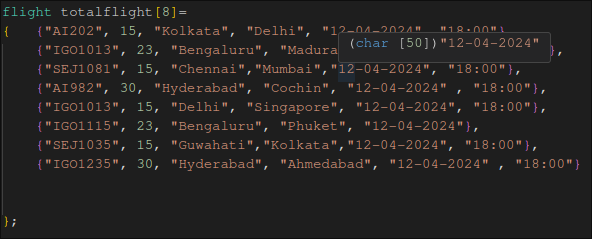
\includegraphics[scale=0.5]{initial.png}
    \caption{Initial List of flights}
\end{figure}
The main project file is \textit{Flight\_Reservation.c} which should be compiled using: 
\begin{center}
    gcc -o Flight\_out Flight\_Reservation.c -lncurses
\end{center}
The \textit{-lncurses} flag is neccessary since we are using the \textit{ncurse.h} library.\\[0.3cm]

\section{Main Structure}
The figure below provides a schematic diagram of the main structure of the program. The arrows indicate the logical flow of the system.
\begin{figure}[H]
    \centering
    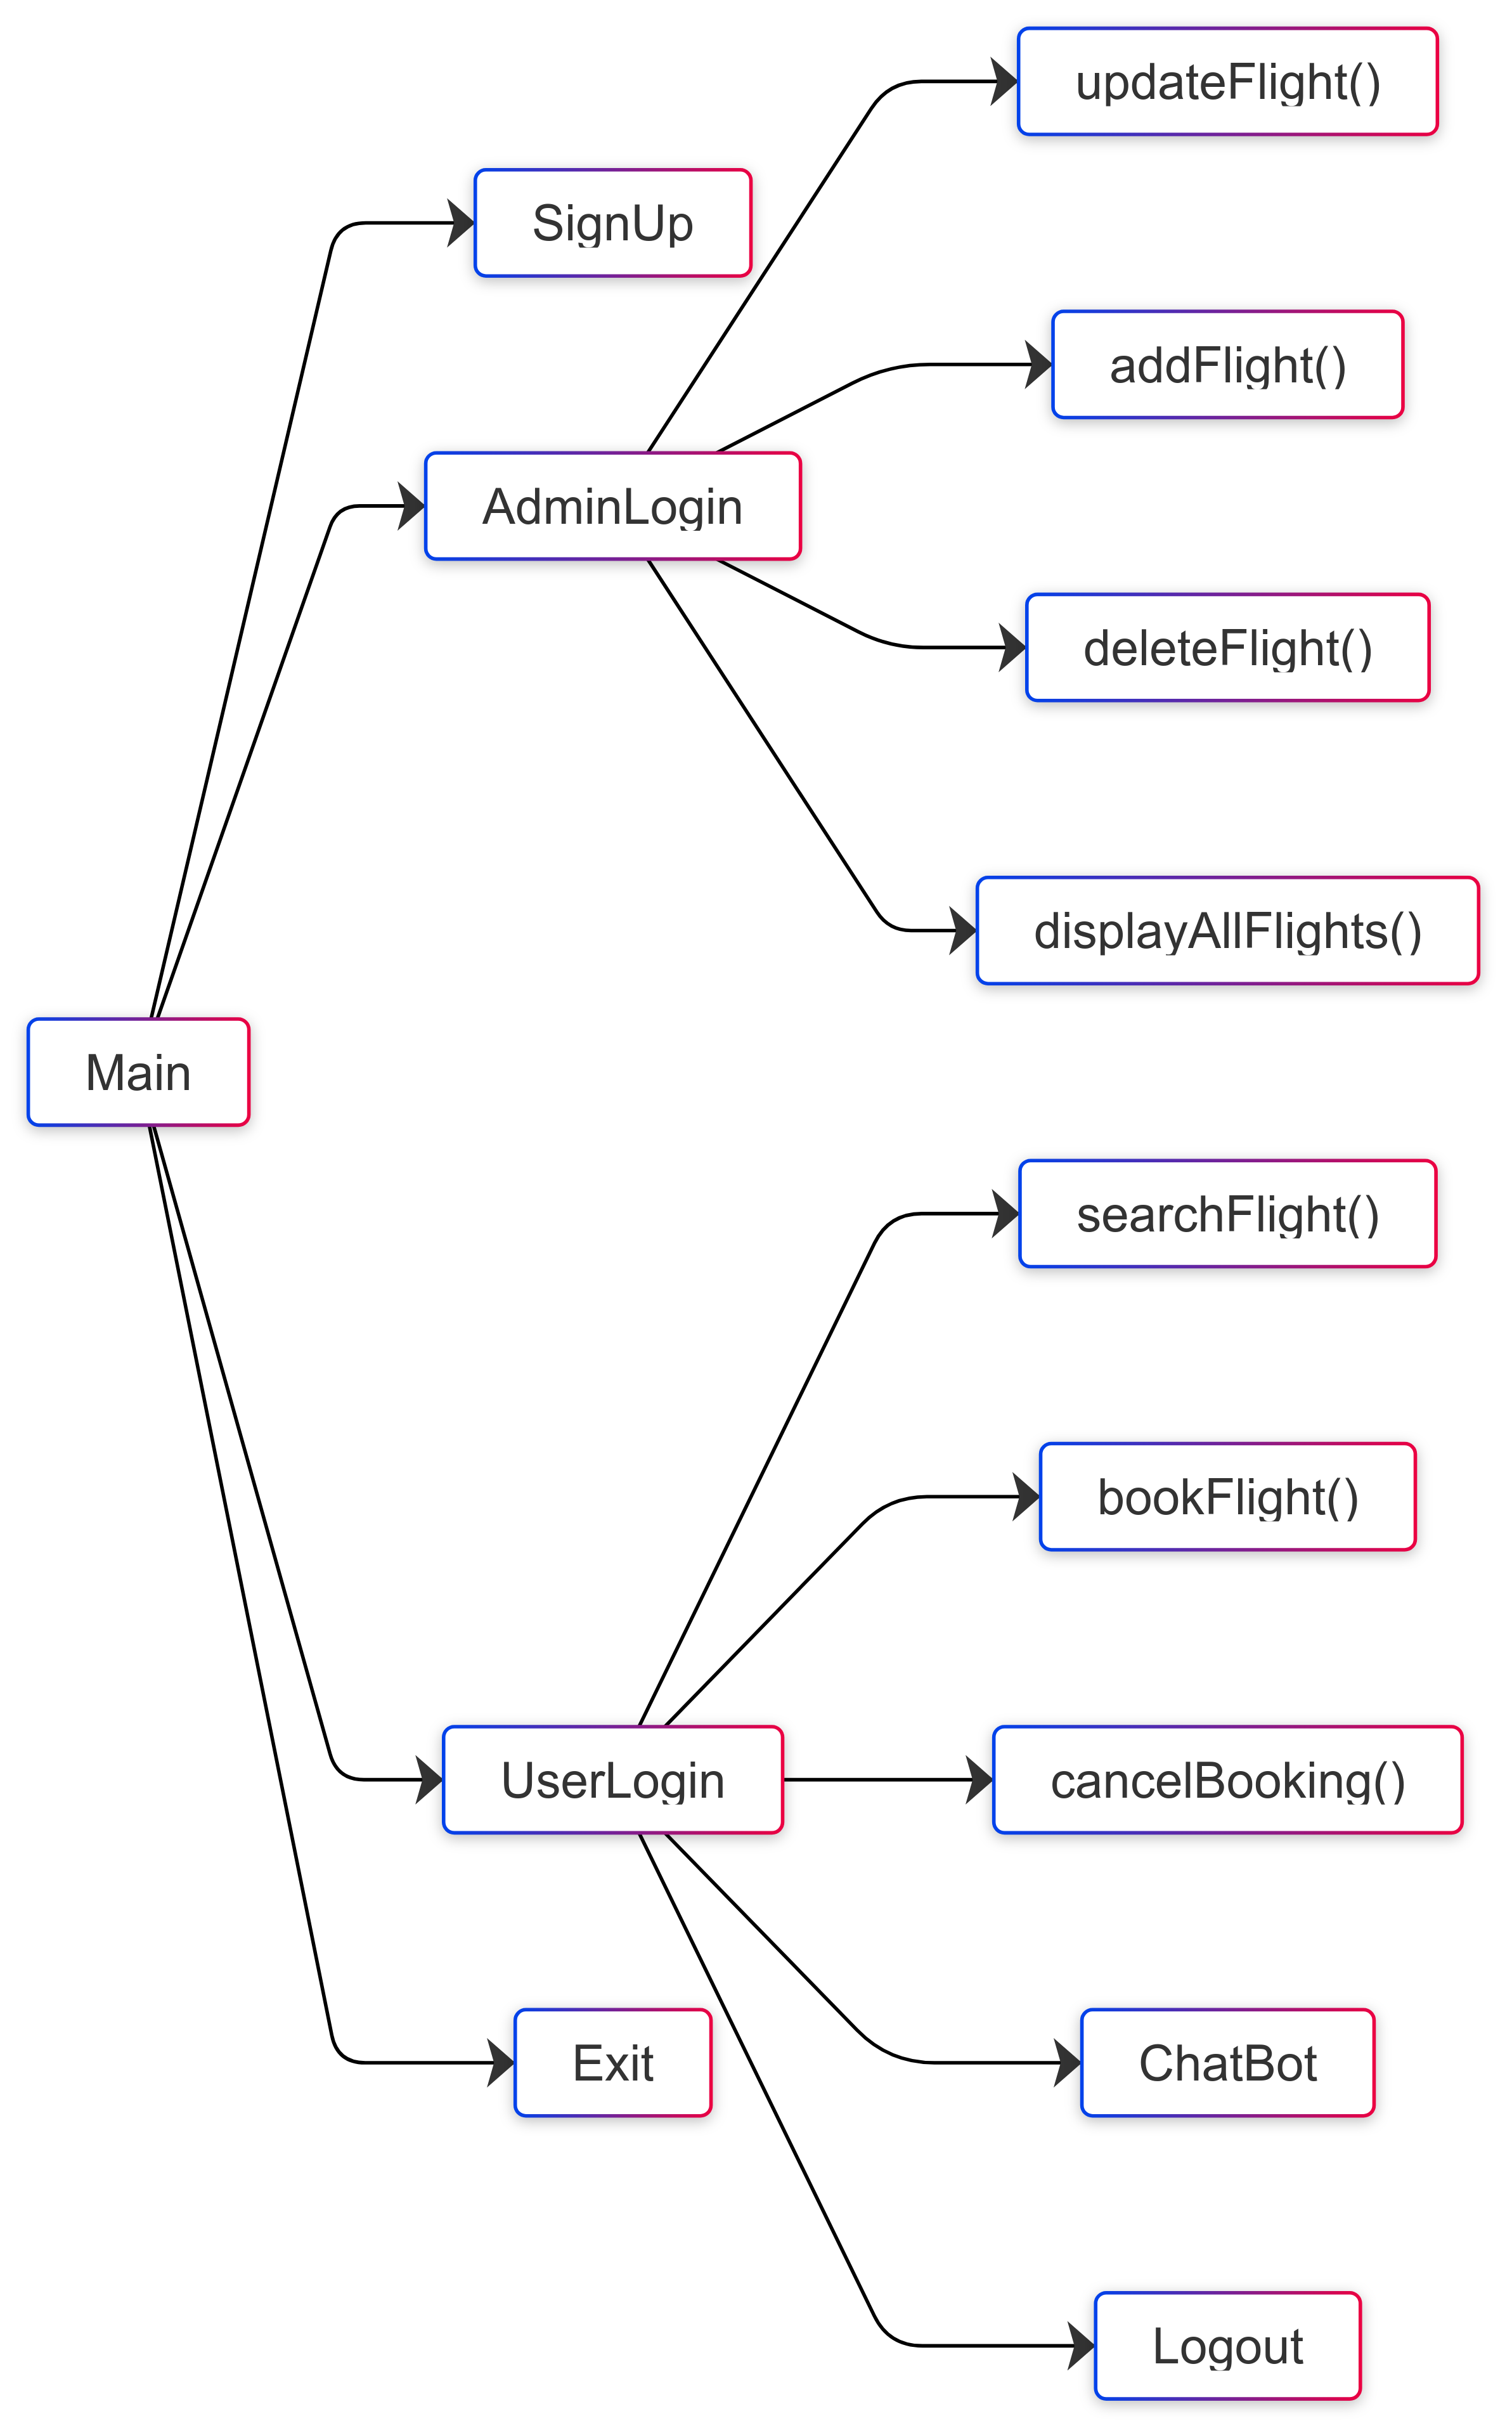
\includegraphics[scale=0.1]{main structure.png}
    \caption{Main structure of the Program}
\end{figure}
\noindent
Starting from the main page, we can either signup (if new user/admin) or login. Accordinly as user/admin, we have the accessibility of different utilitites. 
\begin{figure}[H]
    \centering
    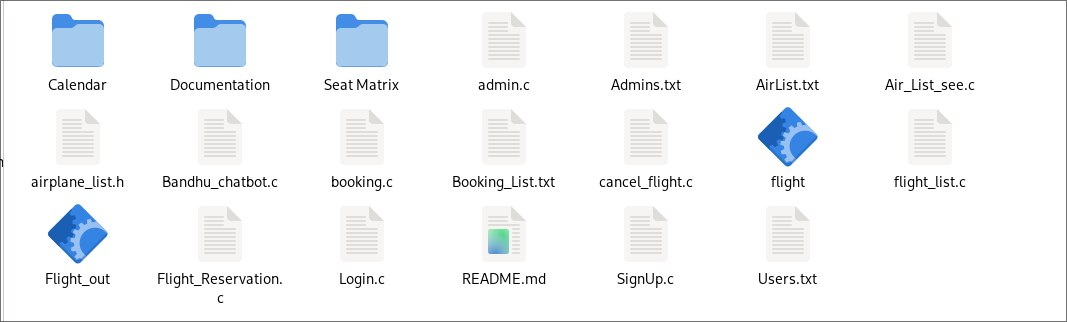
\includegraphics[scale=0.5]{content.jpg}
    \caption{Main contents of the directory}
\end{figure}
\section{Documentation}
\subsection{General Functions}
Functions in Login.c file:
\begin{itemize}
    \item \texttt{int admin\_login()}: This function is used to login as an admin. The admin is asked to enter the username and password. If the username and password match, the admin is redirected to the admin utilities page.\\
    \item \texttt{int user\_login()}: This function is used to login as a user. The user is asked to enter the username and password. If the username and password match, the user is redirected to the user utilities page.\\
\end{itemize}
Functions in SignUp.c: \\[0.2cm]
\texttt{int signup()}: This function is used to signup as a user. The user is asked to enter the username and password. The function then adds the user to the database.\\



\subsection{Functions for User Utilities}
The main Functions used in the User Utilities (contained in the booking.c file) are as follows:
\begin{itemize}
    \item  \texttt{int searchFlight()}: This function is used to search for flights according to the source, destination, date. The function then searches for the flights according to the user's input and displays the flights available.\\
    The function first displays a calendar where the dates available are highlighted in green. Then the user is asked to select the source and destination of his choice and the date of travel. If a flight is found, the user is redirected to the booking page. 

    \begin{figure}[H]
        \centering
        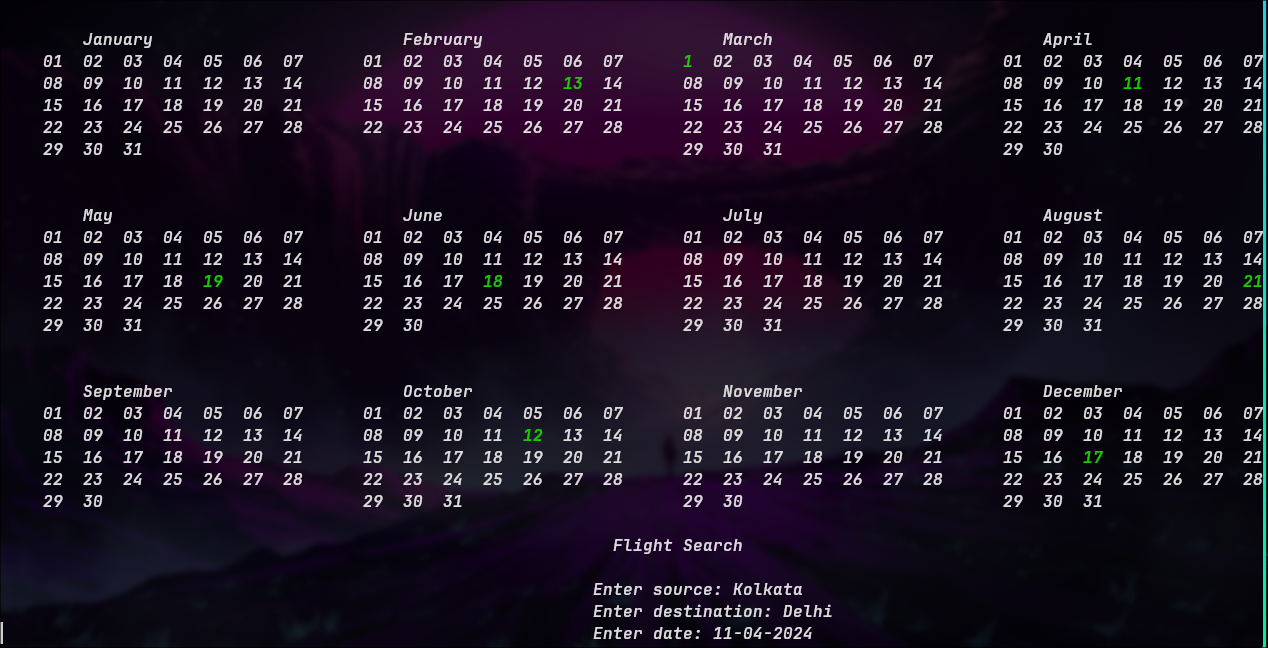
\includegraphics[scale=0.5]{search.png}
        \caption{Contents when search function is called}
    \end{figure}
    \item \texttt{int bookFlight(char* flightnum, char* usr)}: This function is used to book a flight. The user is asked to enter the flight number and the number of seats to be booked. The function then books the flight and updates the booking history. The final bill is then generated and booking is successful\\
    \begin{figure}[H]
        \centering
        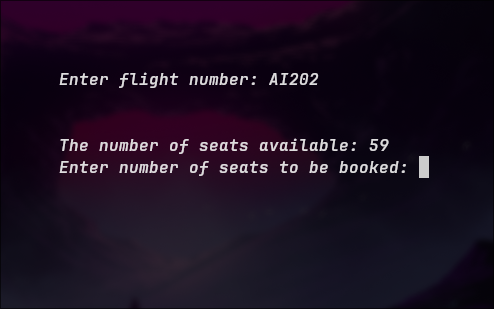
\includegraphics[scale=0.3]{book1.png}
    \end{figure}
    \begin{figure}[H]
        \centering
        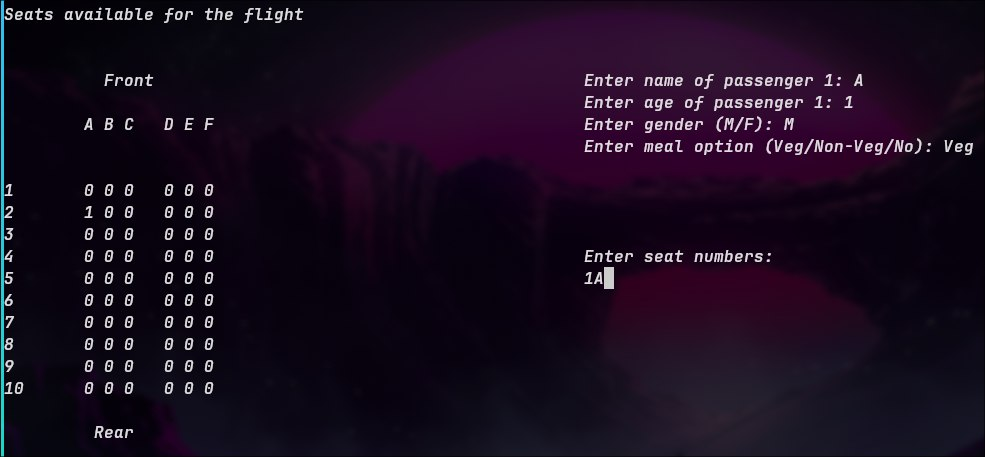
\includegraphics[scale=0.4]{book2.jpg}
        \caption{Contents when booking function is called}
    \end{figure}
    \item \texttt{int cancelBooking(char* tick)}: This function is used to cancel a booking. The user is asked to enter the booking ID and the function then cancels the booking. If a record is found, the user is asked for confirmation of cancellation and the booking is subsequently cancelled. \\
    \item \texttt{void view\_booking\_history()}: This function is used to view the booking history. The function displays the booking record of the user.\\
    \item \texttt{void update\_seat\_matrix(char* filename, char* airnum, char seats[][10], int size, char* mode)}: This function is used to update the seat matrix. The function takes the filename, flight number, the list of seats, the number of seats, the size of the matrix and the mode as input (``add" or ``remove") and updates the seat matrix.\\
\end{itemize}
\subsection{Functions for Admin Utilities}
The main Functions used in the Admin Utilities (contained in the admin.c file) are as follows:
\begin{itemize}
    \item \texttt{void addFlight()}: This function is used to add a flight. The admin is asked to enter the flight details and the function then adds the flight to the database.\\
    \item \texttt{void updateFlight()}: This function is used to update the details of a flight. The admin is asked to enter the flight number and the function then updates the details of the flight.\\
    \item \texttt{void deleteFlight()}: This function is used to delete a flight. The admin is asked to enter the flight number and the function then deletes the flight from the database.\\
    \item \texttt{void displayAllFlights()}: This function is used to display all the flights available. The function displays all the flights available in the database.\\
\end{itemize}
\subsection{Functions for Bandhu--the chatbot}
The code for the chatbot is included in the file  \texttt{Bandhu\_chatbot.c} . The main Functions used in the chatbot are as follows: 

%\begin{itemize}
\noindent
    
\begin{itemize}
    \item \texttt{char *lowering(char *str)}: This function is used to convert a string to lowercase. The function takes a string pointer as input and returns the string in lowercase.
    \item \texttt{const char *keyword\_match(const char *keywords[], char *response, int size)}: This function is used to match the user's input with the keywords array. The function takes the keywords, the user's input and the size of the array of keywords array as input and returns the matched keyword from the array.
    \item \texttt{int indexOf(const char *str[], const char *substr, int size)}: This function is used to find the index of a string in an array of strings. The function takes the array of strings, the string and the size of the array as input and returns the index of the string in the array.
    \item \texttt{int chat(char *name)}: This function is used to chat with the chatbot. The function takes the user's name as input and then provides responses according to user's input.\\
    Various arrays of keywords of different categories like booking, cancellation, greeting, etc. are used in the chatbot. The user provides a response and the function finds whether any word from the various keywords array is a substring of the user's input. If a keyword is found, the chatbot provides a response accordingly.
\end{itemize}
\subsection{Structures:}
We have used different structures to construct the project. The main structures used are:
\begin{itemize}
    \item For defining flight
    \begin{lstlisting}[language=C]
        typedef struct{
        char flightnum[50];
        int seatsFree;
        char source[100];
        char destination [100];
        char date[50]; 
        char time[50];
        double adult_price;
        double child_price;
        double infant_price;
        
        } flight;
    
        
    \end{lstlisting}
    \item For defining a person who is booking the flight
    \begin{lstlisting}[language=C]
        typedef struct {
        char username[50];
        char name[50];
        int age;
        char gender[10];
        char type[10];// determines whether infant or child or adult
        char meal[20];
        char pnr[20];
        char seat[20];
        char flightnum[20];
        double price;
    } BOOKER;

    \end{lstlisting}
    \item For defining the user
    \begin{lstlisting}[language=C]
        typedef struct user{
        char name[50];
        char pwd[50];
        }USER;
    \end{lstlisting}
    \item For defining the admin
    \begin{lstlisting}[language=C]
        typedef struct admin{
        char name[50];
        char pwd[50];
        char id[50];
        }ADMIN;
    \end{lstlisting}
\end{itemize}






\section{Limitations and Future Prospects}
The following are the limitations on which we have to work on:
\begin{itemize}
    \item Adding flights on the same date(but of different months) is not reflected in the calendar due to some array indexing issues.
    \item Choosing the 10th row of the seat matrix provides an error because of double digit issues.
    \item The Chatbox is limited to a few soecific queries and responses containing multiple keywords cant be segregated.
\end{itemize}
\section{Contributions}
The project is a collaborative effort of all the members. We have tried to divide our work equally amongst the members Sagnik and Ronit while Aviyank has mainly worked on the chatbot. 
The contributions from each member are as follows:

\begin{itemize}

    \item \textbf{Ronit Bhuyan} : Worked in the implementation of the admin utilities,like adding , updating and deleting a flight. In the user utilities section, has partial contributions to searching and booking flights. In addition to that, helped in alignment of text and user outputs as well as the documentations.
    
    \item \textbf{Sagnik Seth} : Has written the code for the signup, login page, partially done the booking tickets for user part, worked on the seat matrix printing, viewing the record of the user, cancelling user tickets, for overall presentation of the interface like printing the calendar and the ASCII arts, partially done the chatbot part, and the documentation.
    
    
    
    \item \textbf{Aviyank Aryan}: Helped in the implementation of the chatbot and  completion of the documentations.
\end{itemize}




\end{document}